\documentclass[11pt,letterpaper]{article}
\usepackage[lmargin=1in,rmargin=1in,tmargin=1in,bmargin=1in]{geometry}
\usepackage{../style/homework}
\usepackage{../style/commands}
\setbool{quotetype}{true} % True: Side; False: Under
\setbool{hideans}{false} % Student: True; Instructor: False

% -------------------
% Content
% -------------------
\begin{document}

\homework{6: Due 10/03}{If you fish can catch nothing, you have still caught a lesson.}{Matshona Dhliwayo}

% Problem 1
\problem{10} You are standing at the corner of 6th and 40th while your friend is standing at the corner of 2nd and 59th.
	\begin{enumerate}[(a)]
	\item How many blocks are you from your friend?
	\item How many blocks are you from your friend `as the crow flies'?
	\item What is your Euclidean distance between you and your friend?
	\item What is your Manhattan distance between you and your friend?
	\end{enumerate} \pspace

\sol We can draw a picture of this to aid in the solutions:
	\[
	\fbox{%
	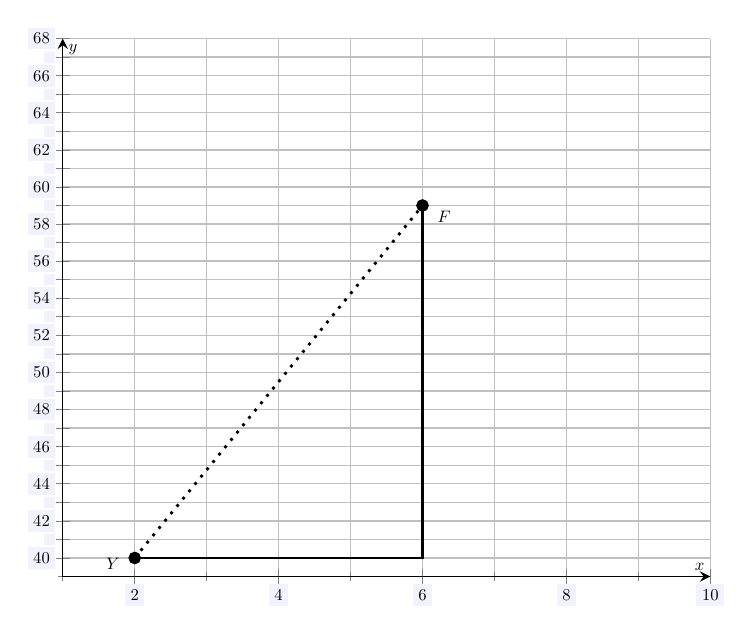
\begin{tikzpicture}[scale=1.2,every node/.style={scale=0.5}]
	\begin{axis}[
	grid=both,
	axis lines=middle,
	ticklabel style={fill=blue!5!white},
	xmin= 1, xmax=10,
	ymin= 1, ymax=30,
	xtick= {2,4,...,10},
	xticklabels={2,4,6,8,10},
	ytick={1,2,...,30},
	yticklabels={39,40,,42,,44,,46,,48,,50,,52,,54,,56,,58,,60,,62,,64,,66,,68},
	minor tick = {1,2,...,10},
	xlabel=\(x\),ylabel=\(y\),
	]
	\node at (1.7,1.7) {$Y$};
	\draw[fill=black] (2,2) circle (0.06cm);
	\node at (6.3,20.4) {$F$};
	\draw[fill=black] (6,21) circle (0.06cm);
	
	\draw[line width=0.03cm] (2,2) -- (6,2) -- (6,21);
	\draw[line width=0.03cm,dotted] (2,2) -- (6,21);
	\end{axis}
	\end{tikzpicture}
	}
	\]

\begin{enumerate}[(a)]
\item Whether we go 6~blocks East and then 19~blocks North, 19~blocks North then 6~blocks East or any combination `in-between', you must travel $4 + 19= 23$ total blocks; that is, you must travel $(6 - 2) + (59 - 40)= 4 + 19= 23$~blocks \pspace

\item This is the `straight line distance (the dotted line above). This is the length of the hypotenuse of a right angled triangle with legs 4 and 19. But then the distance is $\sqrt{4^2 + 19^2}= \sqrt{16 + 81}= \sqrt{97} \approx 9.84886$~blocks. 

\item This is the straight line distance that we computed in (b). Being more formal, we have\dots
	\[
	d= \sqrt{(6 - 2)^2 + (59 - 40)^2}= \sqrt{4^2 + 19^2} = \sqrt{16 + 81}= \sqrt{97} \approx 9.84886 \text{ blocks}
	\]

\item This is the `block' distance we computed in (a). Being more formal, we have\dots
	\[
	|6 - 2| + |59 - 40|= |4| + |19|= 4 + 19= 23 \text{ blocks}
	\]
\end{enumerate}



\newpage



% Problem 2
\problem{10} You see a plane at cruising altitude (approximately 38,000~ft) flying over a nearby airport. You know that the airport is 8.5~mi away. How far is the plane from you at this moment? [5,280~ft $=$ 1~mi] \pspace

\sol First, we compute the cruising altitude to miles: \par
	\begin{table}[!ht]
	\centering
	\begin{tabular}{r|r}
	38000~ft  & 1~mi \\ \hline
			& 5280~ft
	\end{tabular}
	= 7.19697~mi
	\end{table}
Drawing a picture, we can see the distance is the hypotenuse of a right angled triangle. We can then use the Pythagorean Theorem.
	\[
	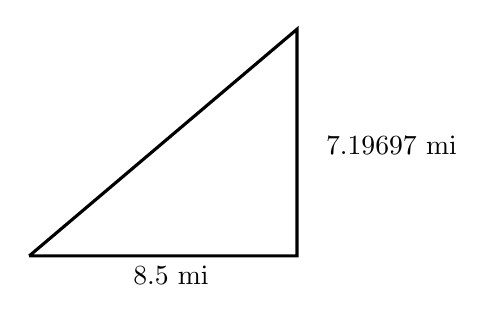
\begin{tikzpicture}[scale=0.4]
	\draw[line width=0.04cm] (0,0) -- (8.5,0) -- (8.5,7.19697) -- (0,0);
	\node at (4.5,-0.6) {8.5~mi};
	\node at (11.5,3.5) {7.19697~mi};
	\end{tikzpicture}
	\]
	\[
	\sqrt{(8.5 \text{ mi})^2 + (7.19697 \text{ mi})^2}= \sqrt{72.25 \text{ mi}^2 + 51.7964 \text{ mi}^2}= \sqrt{124.046 \text{ mi}^2} \approx 11.1376 \text{ mi}
	\]



\newpage



% Problem 3
\problem{10} Suppose you are designing a custom fish tank. The fish tank will be a rectangular box will be 36~in x 18~in x 19~in. The top will be open so that the tank can be accessed. 
	\begin{enumerate}[(a)]
	\item If you have to cover the exposed sides with a special plastic coating, what is the area of plastic coating that is needed per tank?
	\item How much water, in gallons, can the tank hold? [1~ft$^3 =$ 7.48052~gallons]
	\item Suppose you are going to put a volcano in the tank, which will have the shape of a right circular cone. If you put the largest possible volcano in the tank, how much water will it then take to fill the tank?
	\end{enumerate} \pspace

\sol
\begin{enumerate}[(a)]
\item This is a rectangular prism. However, because the top is open, it does not contribute to the area because there is no surface there. Moreover, because the bottom of the tank sits on a table, it also does not need to be covered. Therefore, the exposed area (surface area) is\dots
	\[
	2lh + 2wh + 0lw= 2(36 \text{ in})(19\text{ in}) + 2(18 \text{ in})(19 \text{ in})= 1368 \text{ in}^2 + 684 \text{ in}= 2052 \text{ in}^2
	\] \pspace

\item This is the volume of the tank. This is $V= lwh= (36 \text{ in})(18 \text{ in})(19 \text{ in})= 12312 \text{ in}^3$. We now need to convert this to gallons: \par
	\begin{table}[!ht]
	\centering
	\begin{tabular}{r|r|r|r|r}
	 12312~in$^3$ & 1~ft 	& 1~ft & 1~ft & 7.48052~gallons \\ \hline
				& 12~in & 12~in & 12~in & 1~ft$^3$
	\end{tabular}
	= 53.2987~gallons
	\end{table} \pspace

\item Because the base of the volcano has to fit in the width or length of the tank, it can have a diameter of at most 18~in (the smaller of 36~in and 18~in). This is the diameter of the circular base. Therefore, it has a radius of $18/2= 9$~in. The largest height of the tank is 19~in. Therefore, the volume of the largest possible volcano is $V= \frac{\pi}{3}\, r^2 h= \frac{\pi}{3} \cdot (9 \text{ in})^2 \cdot 19 \text{ in} \approx  1611.64$~in$^3$. Because the volcano will take up this volume, the remaining volume of the tank can be filled with water. This volume is $12312 \text{ in}^3 - 1611.64 \text{ in}^3= 10700.4 \text{ in}^3$. In gallons, this is\dots \par
	\begin{table}[!ht]
	\centering
	\begin{tabular}{r|r|r|r|r}
	 10700.4~in$^3$ & 1~ft 	& 1~ft & 1~ft & 7.48052~gallons \\ \hline
				& 12~in & 12~in & 12~in & 1~ft$^3$
	\end{tabular}
	= 46.3221~gallons
	\end{table} 
\end{enumerate}



\newpage



% Problem 4
\problem{10} Suppose a courtyard at some hedge fund is approximately elliptical in shape. It is approximately 50~ft `the long way' and 35~ft `the short way.'
	\begin{enumerate}[(a)]
	\item What is the area of the courtyard?
	\item If someone can push mow approximately 320~square foot of lawn per minute, how long does it take to mow the courtyard?
	\item If every 1,000~square foot has to be fertilized with 10~lbs of fertilizer and the fertilizer costs \$2.08 per pound, how much does it cost to fertilize the courtyard?
	\end{enumerate} \pspace

\sol 
\begin{enumerate}[(a)]
\item The area of the courtyard is $A= lw= (50 \text{ ft})(35 \text{ ft})= 1750 \text{ ft}^2$. \pspace

\item We know net change, $C$, is related to a constant rate, $r$, and time, $t$, via $C= rt$. We know that the net change of mowed lawn we want is 1750~ft$^2$. The rate at which the lawn can be mowed is 320~ft$^2$/min. But then we have\dots
	\[
	\begin{aligned}
	C&= rt \\[0.3cm]
	1750 \text{ ft}^2&= (320 \text{ ft}^2/\text{min}) t \\[0.3cm]
	t&= 5.46875 \text{ min}
	\end{aligned}
	\]

\item We know that the courtyard is 1750~ft$^2$. Each 1,000 square foot must contain 10~lbs of fertilizer. But then the amount of pounds of fertilizer required per square foot is $10 \text{ lb}/1000 \text{ ft}^2= 0.01 \text{ lb}/\text{ft}^2$. Using $C= rt$, we know that the courtyard requires $1750 \text{ ft}^2 \cdot 0.01 \text{lb}/\text{ft}^2= 17.5 \text{ lb}$ of fertilizer. Each pound of fertilizer costs \$2.08. Therefore, again using $C= rt$, the total cost of 17.5~lb of fertilizer is $17.5 \text{ lb} \cdot \$2.08/\text{lb}= \$36.40$. 
\end{enumerate}


\end{document}